\relatorio
{Consultoria FRST Falconi - Aplicações de simulação de Monte Carlo}
{
    \noindent Pesquisadores: 
    Arthur Pioli,
    Felipe Bakowski,
    Thomas Lipsky,
    Ykaro Andrade
    
    \noindent Orientador: José Renato Garcia Braga
}
{
   Este artigo utiliza métodos estatísticos para investigar frequência de acesso de usuários em uma plataforma para a empresa FRST – Falconi. O objetivo desta foi utilizar as teorias de Cadeia de Markov e Monte Carlo (MCMC) a fim de simular e obter a probabilidade de um usuário transicionar de uma página para um estado de abandono na página, por meio de uma análise de comportamento realizada sabendo, previamente, as probabilidades estacionárias de cada estado. Este estudo é relevante para a FRST- Falconi pois viabiliza um entendimento de quais áreas do site podem ser redesenhadas, mantidas ou excluídas. 
}

\section{Introdução}

    Durante o semestre 2023.2, o Insper Data, em parceria com a FRST Falconi, realizou um projeto cuja finalidade era obter uma análise aprofundada do comportamento de usuários na plataforma própria da FRST utilizando a metodologia das Cadeias de Markov, que fornece um amparo teórico para modelar processos estocásticos. Como resultado deste projeto, os resultados fornecem um modo mais simples de identificar o comportamento dos usuários na plataforma para entender quais etapas no processo de navegação do usuário poderiam se beneficiar de uma mudança ou um redesenho da usabilidade da interface. Além disso, foi possível realizar cálculos dos modelos estacionários das Cadeias de Markov da plataforma e entender onde há maior índice de abandono dos usuários na página.

Ainda, a FRST enfrenta o problema de que não existe uma maneira objetiva de diagnosticar onde pode haver melhorias no âmbito de User Experience - UX. Assim, essa análise visa criar um sistema em que é possível identificar as variações de engajamento dos usuários, a fim de garantir uma melhor experiência para a equipe de desenvolvedores da FRST identificarem possíveis problemas na plataforma e para os usuários.

Com o intuito de realizar uma estimativa mais precisa com os resultados obtidos anteriormente, sem uma limitação de somente uma Cadeia de Markov, mas uma simulação de Monte Carlo aplicada à Cadeia (MCMC) consegue obter resultados mais precisos e aplicáveis ao cotidiano da FRST. Ao aplicar a simulação às Cadeias de Markov, obtém-se uma função distribuição de probabilidade (fdp), justamente da possibilidade da MCMC de prever o comportamento de diversos usuários, a partir de probabilidades estacionárias obtidas por modelos inferenciais.

O objetivo do projeto é dado a partir do momento em que a simulação consegue obter a fdp do sistema da FRST, sendo possível, assim, obter uma avaliação mais precisa da sensibilidade do sistema para mudanças nos parâmetros que o compõem. Com este resultado, consegue-se prever o comportamento futuro deste sistema, utilizando as variações de sensibilidade, e quantificar as probabilidades dos novos estados possíveis.

Na FRST, hodiernamente, todas estas análises são realizadas manualmente e, como não há uma base de dados grande o suficiente para quantificar todas as variações em estados estacionários sem um MCMC, o algoritmo para análise se faz uma ferramenta imprescindível para a realização de mudanças em uma plataforma que necessita de um fluxo constante de novos conteúdos e features. A realização de uma análise de usuários mais consistente consegue resolver esta necessidade da FRST provendo cálculos mais precisos por meio de simulações.


\section{Cadeias de Markov}

A cadeia de Markov é um processo estocástico que evolui ao longo do tempo, passando por diversos estados. A sequência de estados é denotada pela coleção de valores, ou seja, é uma sequência de variáveis aleatórias dependentes. Em uma cadeia de Markov o único estado que importa é o anterior, dessa forma para determinar a sequência de valores que a cadeia pode assumir, podemos determinar a distribuição do próximo valor conhecendo apenas o valor anterior. A coleção de estados que uma cadeia de Markov pode visitar é chamada de espaço de estados. A distribuição de probabilidade condicional, que determina se a cadeia se move de um estado para o outro, é chamada de kernel de transição ou matriz de transição. A seguir tem-se uma representação gráfica de uma Cadeia de Markov: 

\begin{figure}
    \centering
    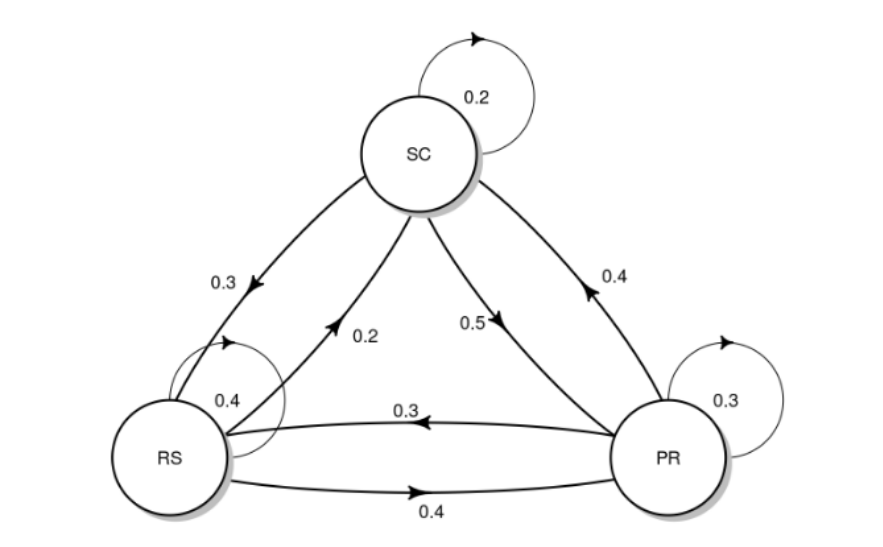
\includegraphics[width = .9\linewidth]{relatorios/frst/figuras/markov.png}
        \caption{Exemplo de Cadeia de Markov}

    \label{fig:mapa}
\end{figure}

\section{Monte Carlo}

    A simulação de monte carlo é aplicada para problemas em que tentamos prever o comportamento de processos aleatórios. Diferente de um modelo de previsão normal, a Simulação de Monte Carlo prevê um conjunto de resultados com base em um intervalo de valores estimados em relação a um conjunto de valores de entrada fixos. Em outras palavras, uma simulação de Monte Carlo cria um modelo de resultados possíveis, usando uma distribuição de probabilidade, como uma distribuição uniforme ou normal, para qualquer variável que tenha incerteza inerente. Ela, então, irá recalcular os resultados sucessivamente, cada vez usando um conjunto diferente de números aleatórios entre os valores mínimo e máximo. Em um teste típico de Monte Carlo, este exercício pode ser repetido milhares de vezes para produzir um grande número de resultados prováveis. A seguir tem-se uma fórmula de uma simulação de Monte Carlo e Cadeia de Markov


\begin{equation}
\label{eq:Fórmula de uma simulação de Monte Carlo e Cadeia de Markov}
    \frac{P_{m}}{P_{n}} = \frac{exp(\frac{-U_{m}}{K_{b}*T})}{exp(\frac{-U_{n}}{K_{b}*T})} = exp(-\frac{U_{m}-U_{n}}{K_{b}*T}) \\
\end{equation}


A equação acima é usada em mecânica estatística ou termodinâmica para descrever a relação entre as probabilidades de um sistema estar em diferentes estados de energia.
 Pm  e  Pn são probabilidades de encontrar o sistema nos estados m e n
Um e Un  são as energias correspondentes a esses estados.
kB é a constante de Boltzmann. T é a temperatura absoluta.
Essa equação é fundamental para entender como a probabilidade de um sistema estar em um certo estado de energia varia com a temperatura e as diferenças de energia.No contexto de MCMC, essa equação pode ser usada para calcular as probabilidades de transição entre estados em um sistema físico.

\section{Aplicação do MCMC}

Métodos de Monte Carlo via Cadeias de Markov (MCMC) consistem em construir uma cadeia de Markov com uma distribuição estacionária desejada e rodar essa cadeia por um longo período de tempo, até que ela se converta (aproximadamente) para essa distribuição estacionária. Os métodos de MCMC são usados basicamente para gerar amostras de uma distribuição que são correlacionadas, especialmente quando a distribuição em questão é complexa ou de alta dimensão.

O ponto principal da MCMC está na formulação de propriedades de transição apropriadas, ou seja, na definição de uma regra de transição que permita à cadeia de Markov explorar eficientemente o espaço de estados e, eventualmente, atingir a distribuição estacionária. Este raciocínio faz muito sentido dentro de uma lógica empresarial e, especialmente, da finalidade que a FRST procura, sendo esta uma busca por prever quais são os estados com maior probabilidade de abandono na plataforma, coisa que a obtenção dos fluxos associados a probabilidades estacionárias conseguem auxiliar a prever, e entender quais são os fluxos dos usuários dentro da plataforma.

\section{Análise teórica}

Para o escopo do projeto, faz-se necessário compreender o fluxo comportamental do usuário no site, ou seja, qual o caminho que um indivíduo percorre dentro da plataforma. Nessa medida, deve-se criar estados e atribuir um número a cada um deles, por exemplo uma página pode equivaler ao estado 3 e a ação de sair do site pode ser o estado 20, e então, pode-se montar uma matriz de transição, a qual descreve as probabilidades de transição em uma cadeia de Markov. Ainda, essa matriz é de suma importância para a análise, pois com ela é possível rodar as simulações de Monte Carlo e obter a função de distribuição de probabilidade para cada cenário. Por último, todas essas variáveis são latentes e não há necessidade de uma variável proxy (variável utilizada para substituir outra de difícil mensuração), pois todas as informações são fáceis de se obter, uma vez que esses dados já foram coletados. 

\section{Análise descritiva}

Para a elaboração e sucesso deste projeto, é fundamental que os dados referentes ao tráfego de usuários em nossa plataforma sejam coletados, armazenados e organizados para a análise. Esses dados originam-se diretamente das interações que os usuários estabelecem com a plataforma - especificamente, através dos cliques efetuados e do tempo despendido em cada página. Tais interações são interpretadas como ações explícitas dos usuários, sendo registradas em detalhe a cada sessão de login. Este processo de coleta permite um mapeamento preciso e individualizado do comportamento de cada usuário, estabelecendo a base para nossa análise.

Cada ação do usuário é catalogada e vinculada ao seu respectivo login, garantindo a fonte de dados para análise. Essas informações são essenciais para definir os "estados" no contexto das Cadeias de Markov, onde cada página visitada na plataforma é considerada um estado possível. A transição de um estado para outro - ou de uma página para outra - é influenciada pela probabilidade baseada no comportamento histórico dos usuários, informações essas que são cruciais para a modelagem através das Cadeias de Markov.

\section{Coleta e Estruturação dos Dados}


A coleta de dados é realizada por meio de ferramentas de tracking embutidas na plataforma, que registram cada clique e o tempo gasto em cada página por usuário. Esses dados são então estruturados em um formato que facilita a aplicação das técnicas de análise mencionadas. A estruturação adequada inclui a categorização das páginas (estados), o mapeamento das transições entre páginas e a quantificação do tempo despendido. Além disso, aspectos como a ordem das visitas às páginas e as ações realizadas em cada uma são detalhadamente registrados, permitindo uma análise granular do fluxo de navegação do usuário.

\section{Visualização dos estados da FRST}

	Após a coleta de dados é possível visualizar os estados de transição (páginas do site) que compõem a cadeia de Markov através de um gráfico de rede, como pode ser visto a seguir: 

\begin{figure}
    \centering
    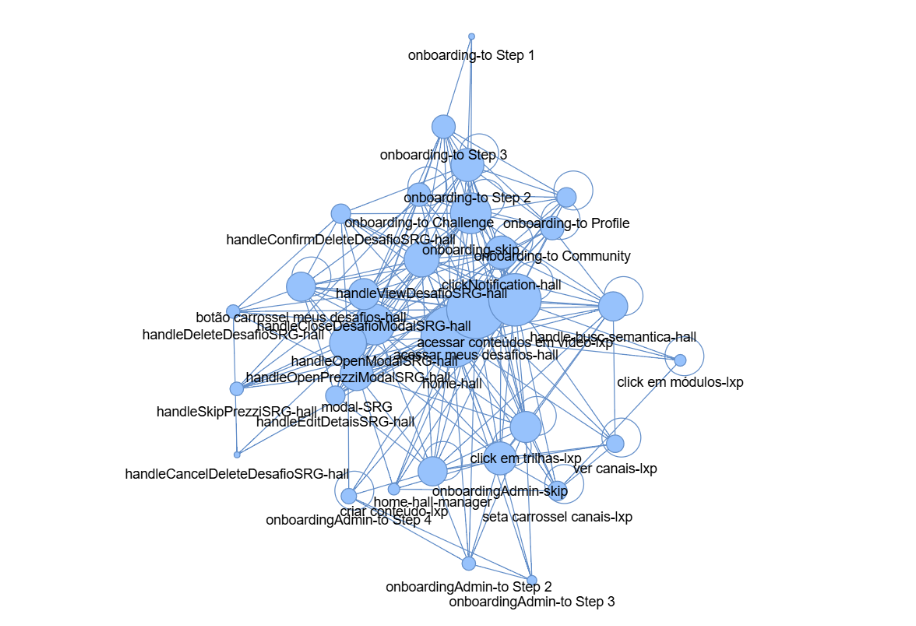
\includegraphics[width = .9\linewidth]{relatorios/frst/figuras/estados1.png}
        \caption{Estados}

    \label{fig:mapa2}
\end{figure}

Este gráfico representa todos os estados do site da FRST com todas as possibilidades de transição entre as páginas e a frequência que os usuários estão em cada página do site, mas como a visualização fica impossibilitada pela quantidade dos estados na cadeia.

\begin{figure}
    \centering
    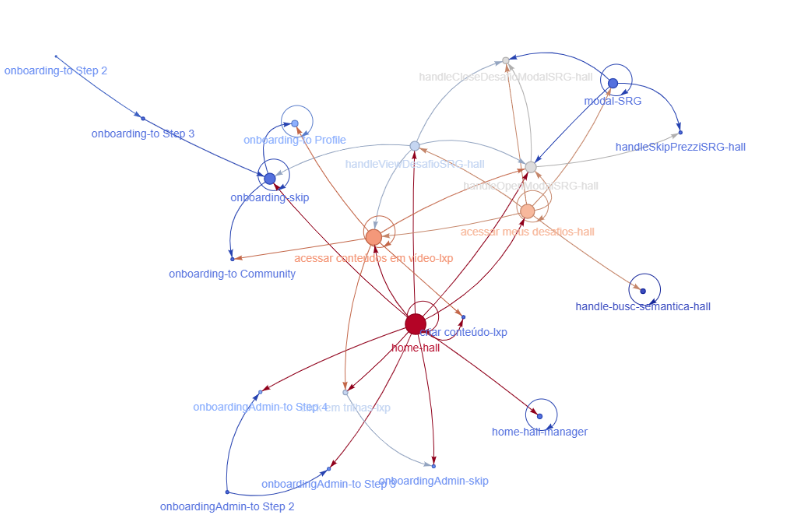
\includegraphics[width = .9\linewidth]{relatorios/frst/figuras/estados2.png}
        \caption{Estados}

    \label{fig:mapa3}
\end{figure}

Cabe pontuar que, esse gráfico é uma fração da base de dados inteira, pois utilizar uma parte menor ajuda na clareza visual, ainda mais que, os estados apresentados nesta visualização simplificada compõem os principais da plataforma da FRST.

\section{Conclusão}


A partir da implementação do método de Monte Carlo, a análise permitirá realizar múltiplas simulações de caminhos de navegação dos usuários pela plataforma, baseando-se nas probabilidades derivadas das Cadeias de Markov. Ao simular inúmeros cenários possíveis, podemos identificar padrões e tendências no comportamento do usuário, fornecendo insights valiosos para otimizações na usabilidade e no design da interface da plataforma FRST.
